\section*{Question 2}

\subsection*{Newton-Raphson}
Soit la fonction $G$ de la question 1. On souhaite appliquer la méthode de Newton pour trouver le point $s$ tel que $G(s)=0$. On a montrer précédemment que $G(y)=0$ ssi  $(w+ W_{\bot}y)$ est un vecteur propre de $A$. La méthode de Newton appliquée à $G$ permet donc bien de trouver le vecteur propre dominant de $A$.
Utilisons le théorème $3.10$ énoncé à la question 1.
Dans notre cas, on voit aisément que $J_G(y) = W_{\bot}^*AW_{\bot} - w^*AwI - (yw^*AW_{\bot}+Iw^*AW_{\bot}y) $ est continu en $s$ ($I$ est la matrice identité de taille $n-1$).

On peut étendre le théorème $3.10$ avec des hypothèses plus forte sur la jacobienne : 

Si, de plus, il existe une constante $\alpha > 0$ telle que la condition de Lipschitz est satisfaite
$$||DF(x) - DF(s)|| \leq \alpha || x - s||, \forall x \in \Omega,$$
alors l'ordre de convergence est au moins 2. 

Dans notre cas, en utilisant l'inégalité de Cauchy et l'inégalité triangulaire, on obtient que : 
\begin{eqnarray}
||DG(x) - DG(s)|| &=& ||W_{\perp}^{*} A W_{\perp}- w^{*} A wI - (xw^*AW_{\bot}+Iw^*AW_{\bot}x) - W_{\perp}^{*} A W_{\perp}+ w^{*} A wI + (sw^*AW_{\bot}+Iw^*AW_{\bot}s) || \\
||DG(x) - DG(s)|| &=&  ||(sw^*AW_{\bot}+Iw^*AW_{\bot}s) - (xw^*AW_{\bot}+Iw^*AW_{\bot}x) || \\
 ||DG(x) - DG(s)|| &\leq & (||w^*AW_{\bot}|| + || Iw^*AW_{\bot} ||) || x-s ||
\end{eqnarray}
Par identification on a $\alpha = ||w^*AW_{\bot}|| + || Iw^*AW_{\bot} || \geq 0$, et donc la condition de Lipschitz sur $DG(x)$ est satisfaite.On conclut qu'on a bien un ordre de convergence d'au moins 2 pour la méthode de Newton appliquée à la fonction $G$.\\

Passons à présent à l'étude numérique de la méthode. Nous séparons notre analyse en trois étapes : (1) la représentation graphique de la méthode pour une matrice $A$ de taille 3; (2) l'étude numérique de la convergence et de la vitesse de convergence de la méthode.

\subsubsection{Étude graphique}
L'interprétation graphique de la méthode de Newton appliqué à la fonction $G$ est la suivante. Contrairement à la question 1.1. où la fonction $F$ calculait un vecteur $x$ de taille $n$ (avec $A$ matrice de taille $n$) qui était le vecteur propre dominant; la fonction $G$ va fixer un vecteur $w$ de tel sorte qu'on ne doivent plus calculer qu'un vecteur $y$ (dans la base $W_{\bot}$ orthogonale à $w$) de taille $n-1$. On "perd" en quelque sorte un degré de liberté. Illustrons cela sur un cas particulier.\\

Soit $A=  \left[ 
\begin{matrix}
1 & 3 & 5 \\
-2 & 4 & 6 \\
5 & 4 & -8
\end{matrix} \right] 
, w = 
\left[ 
\begin{matrix}
1 \\
0\\
0
\end{matrix} \right] , 
W_{\bot} = 
\left[ 
\begin{matrix}
0 & 0 \\
1 & 0 \\
0 & 1 
\end{matrix} \right] , 
Q=
\left[ 
\begin{matrix}
0.2672 & 0.9094 & 0.7416 \\
0.3831 & -0.2059 & 0.5256 \\
-0.8842 & 0.3613 & 0.4169
\end{matrix} \right] 
$\\
Où $Q$ est la matrice des vecteurs propres de $A$. Les vecteurs propres sont donc des vecteurs de l'espace $\mathbb{R^3}$ (cf. figure \ref{figureNewton}). $W_{\bot}$ est un plan de normale $w$. La méthode recherche un vecteur $y$ qui appartient au plan $W_{bot}$. Ou encore $y_1$, $y2$, $y3$ sont les projections orthogonale de $v1$, $v2$ et $v3$ dans le plan $W_{\bot}$.

\begin{figure}
\centering
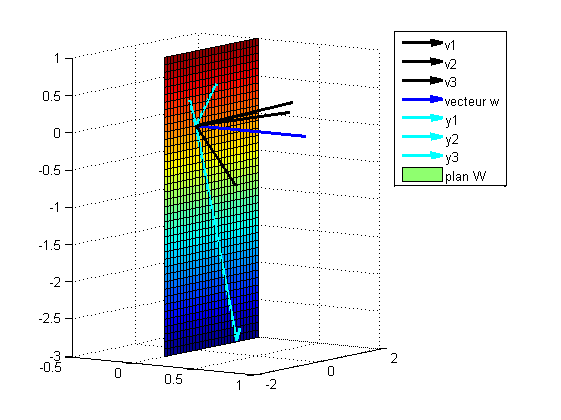
\includegraphics[width=12cm]{grapheNewton.png}\\
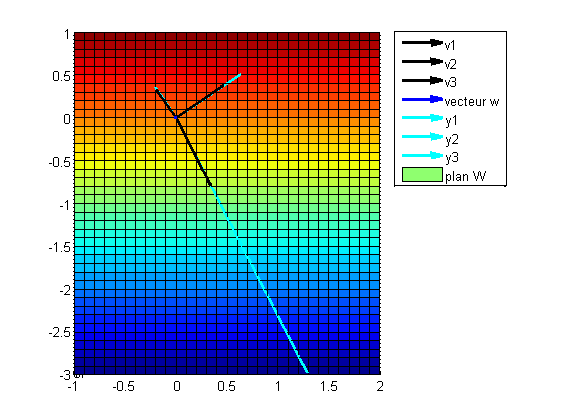
\includegraphics[width=12cm]{grapheNewton2.png}
\caption{Illustration graphique de la méthode de Newton appliquée à la fonction $G$. Le vecteur bleu est $w$ qui ets fixé. La méthode va chercher un $y_1$ (resp. $y_2$ ou $y_3$) tel que la somme vectorielle $w+y_1$ soit le vecteur propre $v_1$ (resp. $v_2$ ou $v_3$).}
\label{figureNewton}
\end{figure}

Si on représente la fonction $G$ pour ces même matrices $A$, $W_{\bot}$ et $w$, on obtient la figure \ref{grapheG}.

\begin{figure}
\centering
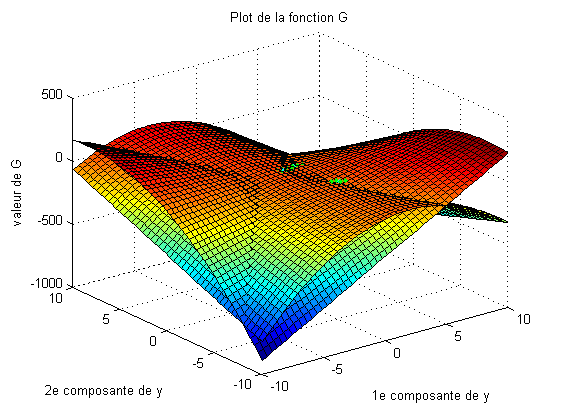
\includegraphics[width=12cm]{grapheG.png}\\
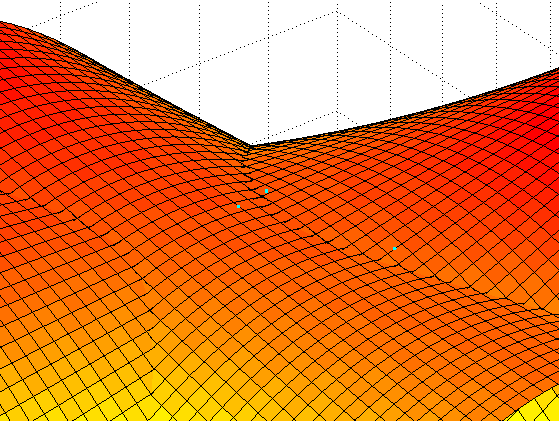
\includegraphics[width=12cm]{grapheG2.png}
\caption{Graphes de la fonction $G$. $G$ étant une fonction vectorielle à deux composante ($G(y)=[G_1(y), G_2(y)]$), nous avons tracer les deux courbes sur un même graphe. On cherche les points $y$ tels que $G_1(y)=G_2(y)=0$. Ces points sont tracer en vert sur les graphes ($G_1$ et $G_2$ étant ici tracer approximativement, ce points ne sont pas tous des racines mais permettent de localiser grossièrement les zones où se trouvent les vraies racines de $G$, ce qui est suffisant pour notre analyse), tandis que les points $y$ sont tracer en blanc.}
\label{grapheG}
\end{figure}
Graphiquement, la méthode de Newton convergera (pas toujours, selon les bassins de convergence de la méthode) vers un $y$ le plus proche de $y_0$, l'itéré de départ.\\



Regardons ce qui se passe quand $w$ est orthogonal au vecteur propre dominant. Cela signifie que $v_1$ est dans le plan $W_\bot$. Par conséquent, on ne peut exprimer $v_1$ par $w+W_{\bot}y$ (sauf peut-être pour $||y|| \rightarrow \infty$). \\
Soit $w = 
\begin{bmatrix}
1 \\
0\\
0.3021
\end{bmatrix} , 
W_{\bot} =  
\begin{bmatrix}
0 & 0.2672 \\
1 & 0 \\
0 & -0.8842 
\end{bmatrix}$\\
La fonction $G$ n'a plus que deux racines (cf. figure \ref{FigNewtonv1inW}).

\begin{figure}
\centering
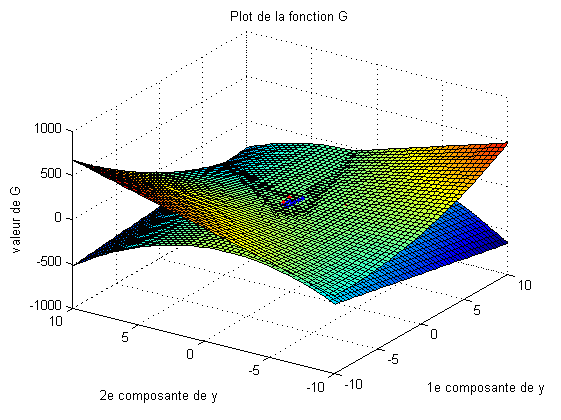
\includegraphics[width=12cm]{grapheG3.png}
\caption{Graphe de $G$ pour la même matrice $A$, mais pour $v_1 \bot w$  
}
\label{FigNewtonv1inW}
\end{figure}


\subsubsection{Étude de la convergence}







\subsection*{Rayleigh symétrique}
On peut voir la méthode de Rayleigh comme une méthode de la puissance avec un "shift" variable (mis a jour à chaque itération). En d'autre mots, elle définie la méthode itérative suivante : 
$$x_{k+1} = \left(  A- \frac{x^*Ax}{x^*x}  \right)^{-1} x_k.  $$
\textbf{Proposition 4.4} Soit $A = A^*$ $ \in \mathbb{C}^{n\times n}$. L'itération du quotient de Rayleigh pour $A$ converge vers une direction propre de $A$ pour presque tout itéré initial. Lorsque la suite des itérés converge vers une direction propre, la convergence est cubique. 

Il faut maintenant préciser ce \textit{pour presque tout itéré initial}. Supposons que $A$ est diagonalisable et faisons un changement de variable afin d'exprimer $x$ dans la base formée par les vecteurs propres de $A$. Nommons le $x$ après changement de variables $x'$. Soit $Q$ la matrice dont les colonnes sont les vecteurs propres de $A$ et $D$ la matrice diagonale des valeurs propres de $A$. On utilise le théorème spectrale et le fait que $A$ et $(A-\mu I)^{-1}$ possèdent les mêmes vecteurs propres pour réécrire l'itération : 
\begin{eqnarray}
Qx_{k+1}' & = &(Q D Q^T - \frac{x_k'^* D x_k}{x_k'^* x_k})^{-1} Qx_{k}'\\
Qx_{k+1}' & = & Q(D-\frac{x_k'^* D x_k}{x_k'^* x_k})^{-1}Q^T Qx_k'\\
x_{k+1}' & = & \underbrace{(D-\frac{x_k'^* D x_k}{x_k'^* x_k})^{-1}}_{\text{matrice diagonale}} x_k'
\end{eqnarray}
Supposons qu'on souhaite converger vers le vecteur propres dominant $v_1$, autrement dit on souhaite que $lim_{k\rightarrow \infty} x_k' = [1 0 \cdots 0]^T$. Pour que cela soit possible, il faut que $x_0$ ait sa composante dans la direction $v_1$ non nulle ($x_0'^* v_1 \neq 0$). 

\subsection*{Rayleigh asymétrique}